%
%  intro.tex
%
%  Created by Drew Conway on 2011-01-26
% 
%
\documentclass[xcolor=dvipsnames, 9pt]{beamer}

\usepackage{amssymb}
\usepackage{amsfonts}
\usepackage{amsmath}
\usepackage{hyperref}
\usepackage{natbib}
\usepackage{color}
\usepackage{pdfsync}
\usepackage{chancery}
\usepackage{movie15}
\usepackage{pgfpages}
\usepackage{fancyvrb}
\usepackage{colortbl}
\usepackage{multirow}

\usepackage{graphicx}
\graphicspath{{../../images/figures/}{../../images/logos/}{../../images/graphs/}/}

\usepackage{beamerthemesplit}
\usetheme{Copenhagen}
\definecolor{title}{RGB}{128,148,182}
\usecolortheme[named=title]{structure} 
\setbeamertemplate{headline}{}
\setbeamertemplate{navigation symbols}{}
\setbeamertemplate{itemize items}[triangle]
\setbeamertemplate{enumerate items}[default]
\setbeamertemplate{footline}[page number]{}
%\setbeameroption{show notes on second screen}


\usepackage{listings}
%\usepackage{listings,arev}
\definecolor{keywords}{RGB}{128,148,182}
\definecolor{comments}{RGB}{60,179,113}
\lstset{numbers=left,
        showstringspaces=false,
        numberstyle=\tiny,
        %frame=leftline,
        numbersep=4.5pt,
  keywordstyle=\color{keywords}\bfseries,
  commentstyle=\color{YellowOrange}\emph
}

\newenvironment{code}{\begin{semiverbatim} \begin{footnotesize}}
{\end{footnotesize}\end{semiverbatim}}


\newcommand{\R}{\mathbb{R}}
\renewcommand{\d}{\mathsf{d}}
\newcommand{\dd}{\partial}
\newcommand{\E}{\mathsf{E}}
\newcommand{\bb}{\mathbf}

\title{Welcome to Data Bootcamp}
\author{Joseph Adler, Drew Conway, Jake Hofman, Hilary Mason}
\date{February 1, 2011}

\begin{document} 
    
\begin{frame}[plain]
  \titlepage 

  \tiny
  \href{http://creativecommons.org/licenses/by-sa/3.0/us/}{
\includegraphics[width=1cm]{ccbysa}}

  Creative Commons Attribution-Share Alike 3.0
\end{frame}

\section{Motivation for Bootcamp} % (fold)
\label{sec:motivation_for_bootcamp}

\begin{frame}[fragile]
    \frametitle{Getting the code}
    All of the slides, code and images from today's tutorial are available on Github:
    \vspace{1cm}
    \begin{center}
        \LARGE{\url{https://github.com/drewconway/strata_bootcamp}}
    \end{center}
    \vspace{1cm}
    \begin{block}{The play the home game}
        \begin{lstlisting}[language=bash]
$ git clone https://github.com/drewconway/strata_bootcamp
        \end{lstlisting}
    \end{block}
\end{frame}

\begin{frame}[fragile]
    \frametitle{The data science ``black box''}
    \begin{center}
        \only<1>{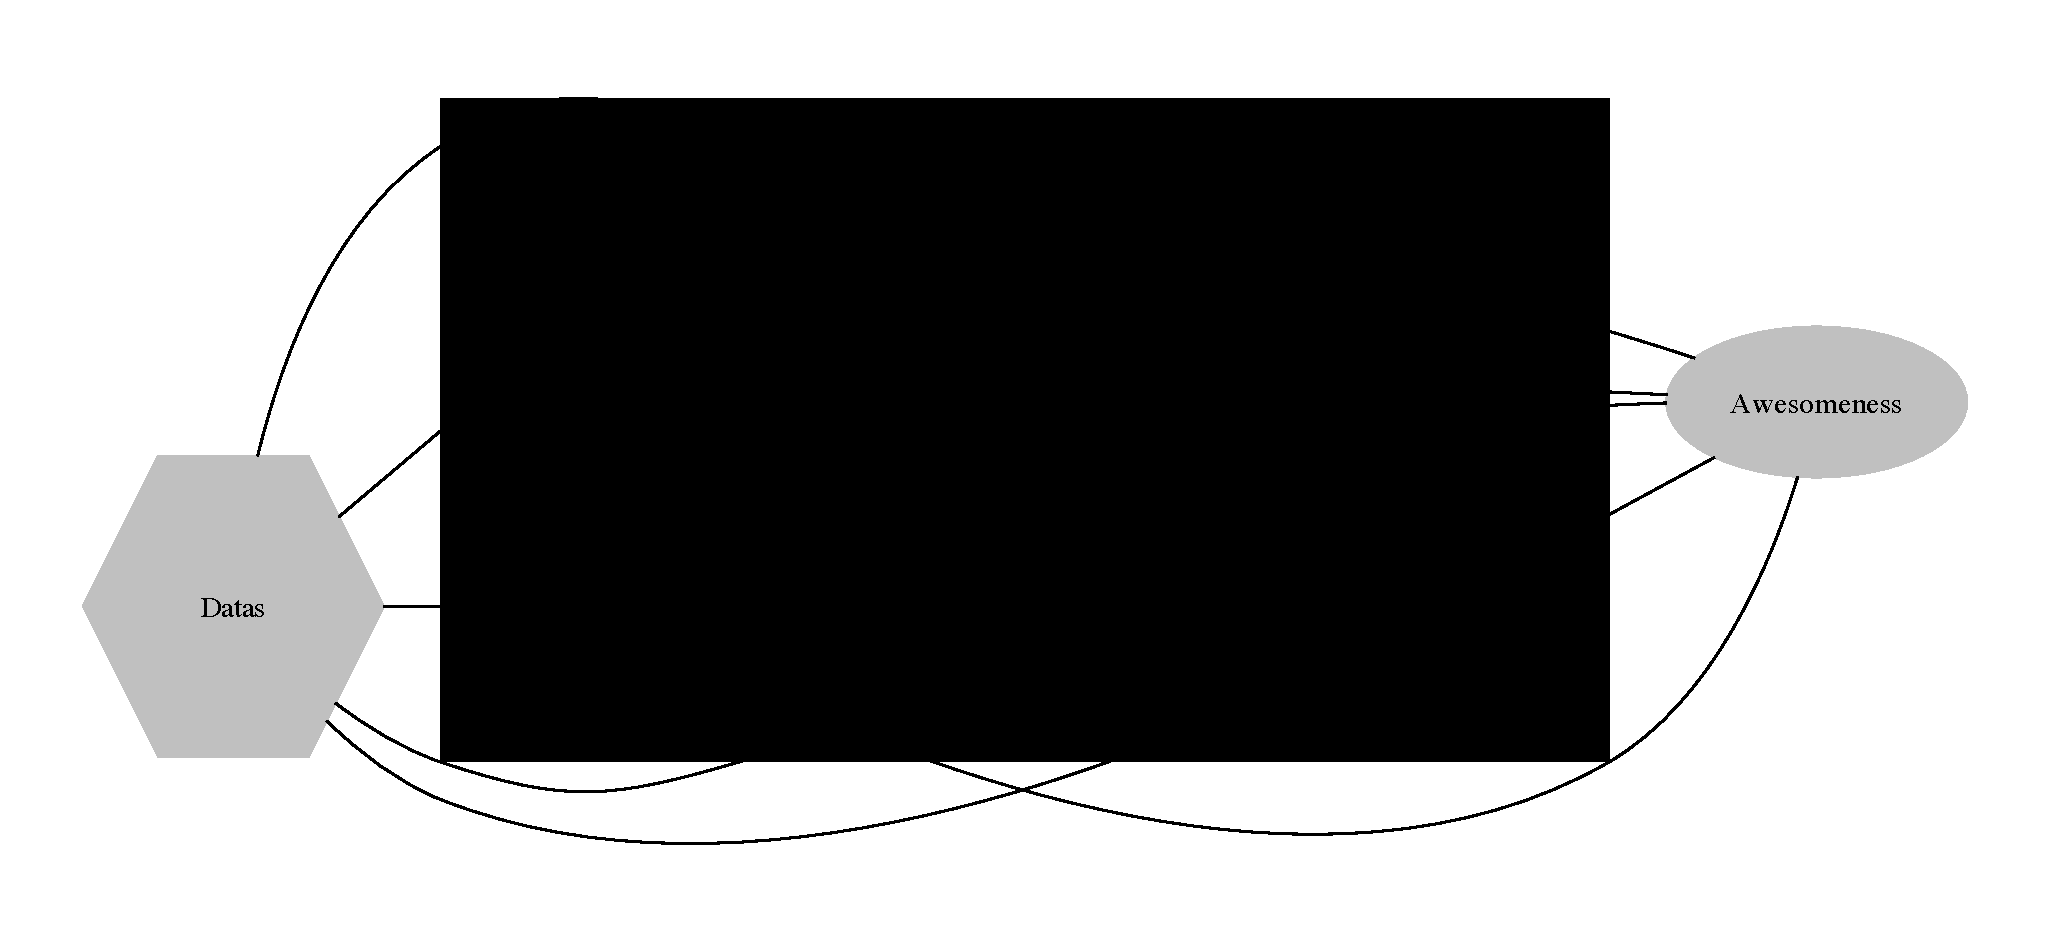
\includegraphics[width=12cm]{black_box.pdf}}
        \only<2>{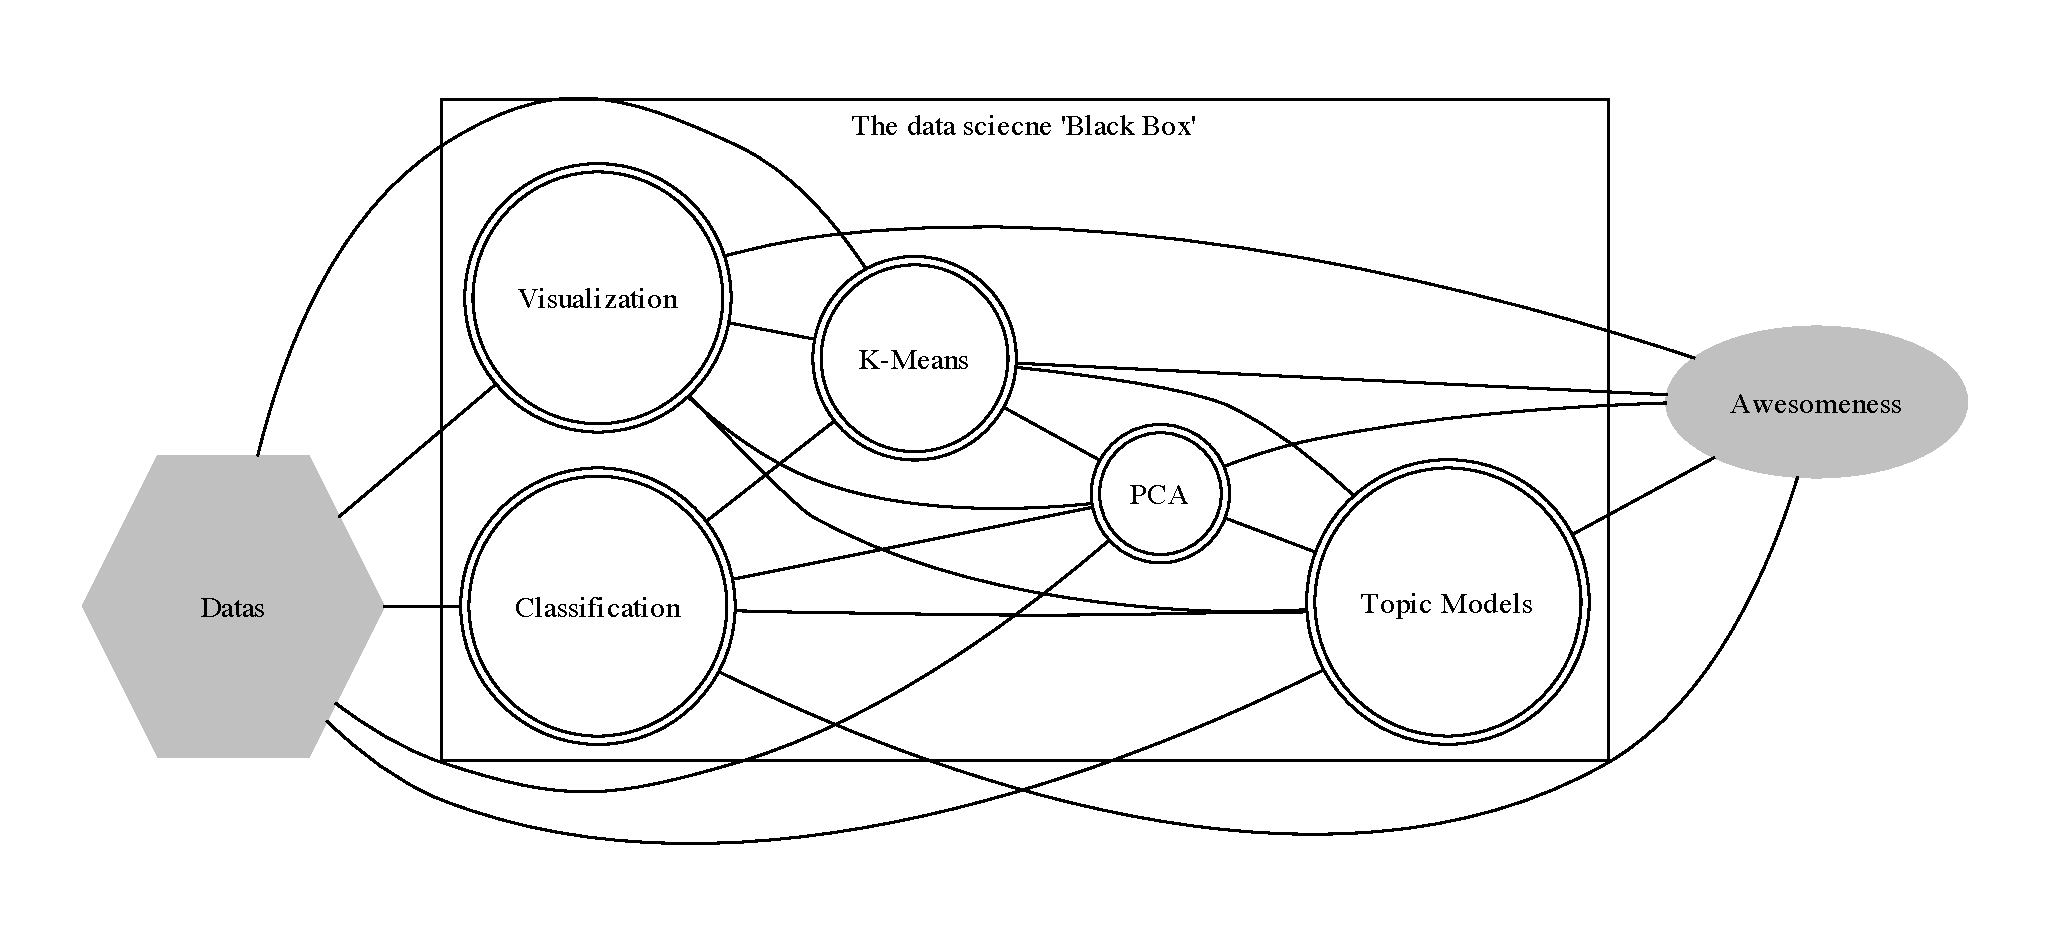
\includegraphics[width=12cm]{black_box_reveal.pdf}}
    \end{center}
\end{frame}

\begin{frame}
  \frametitle{Learning by example}

    \begin{center}
      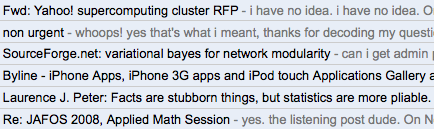
\includegraphics[width=0.75\textwidth]{email_ham.png}
      
\includegraphics[width=0.75\textwidth]{email_spam.png}
    \end{center}

    \begin{itemize}
      \pause
      \item How did you solve this problem?
      \item \alert<2>{Can you make this process explicit (e.g. write code to do so)?}
    \end{itemize}

\end{frame}


\begin{frame}
  \frametitle{Learning by example}

    \begin{center}
      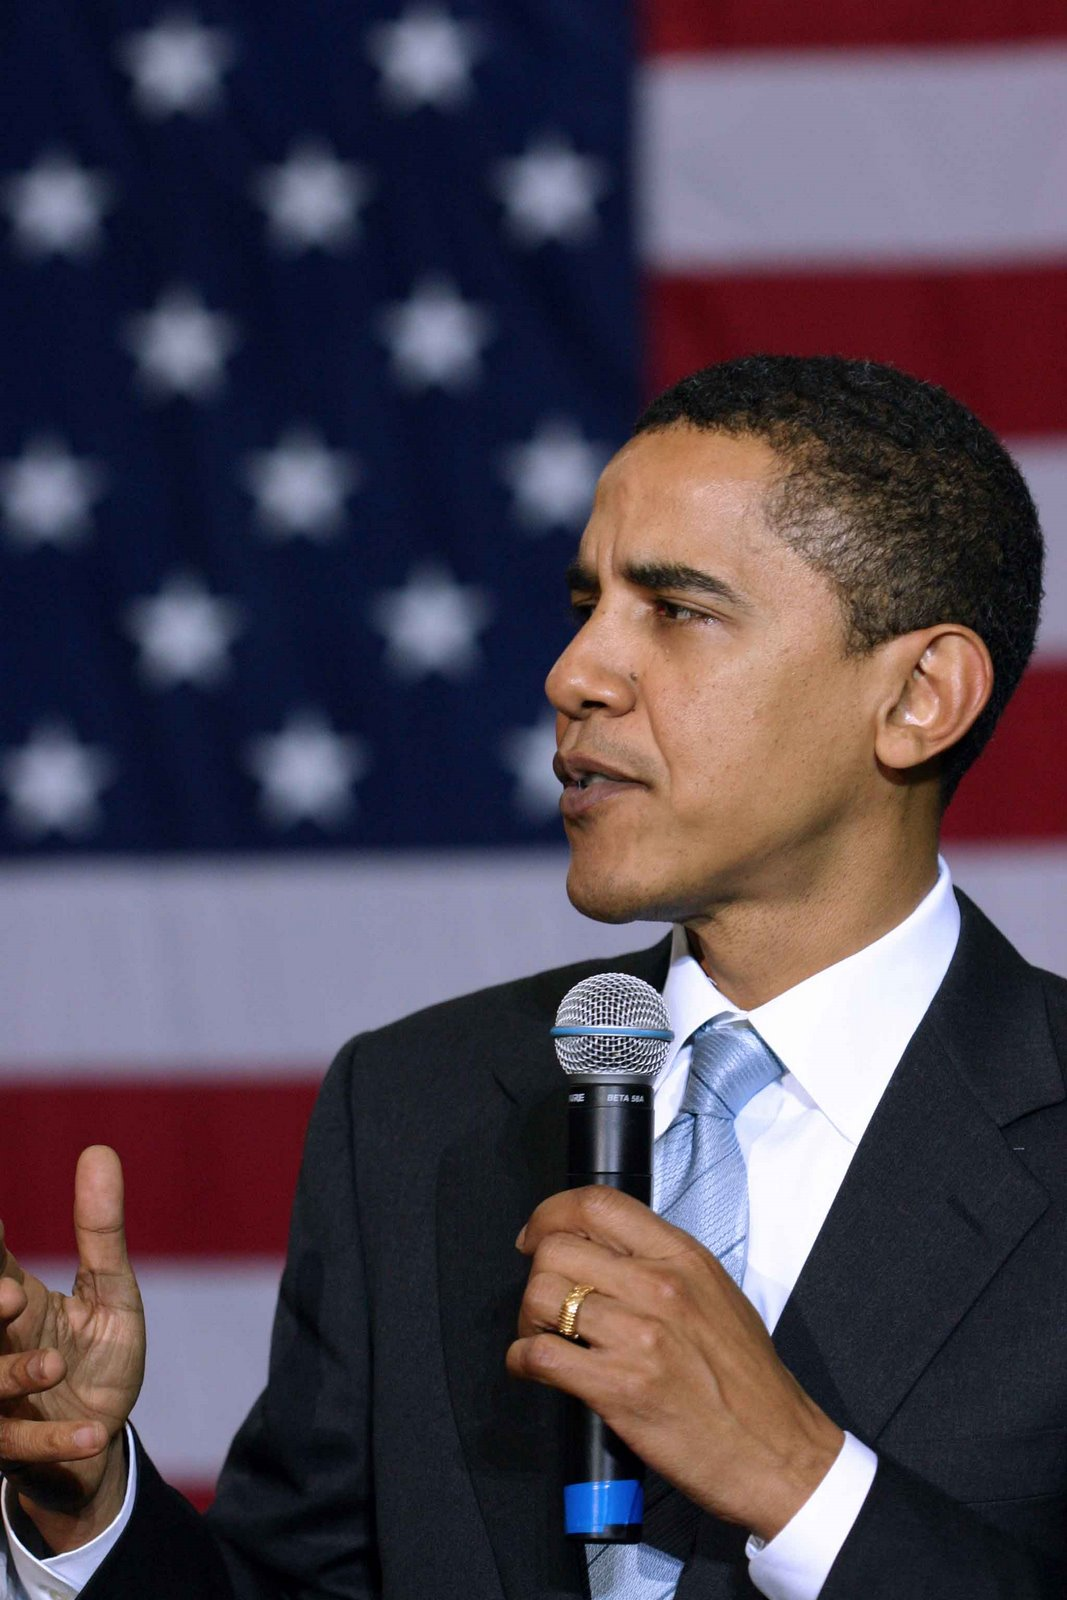
\includegraphics[width=0.25\textwidth]{obama1.png}
      
\includegraphics[width=0.25\textwidth]{obama2.png}
      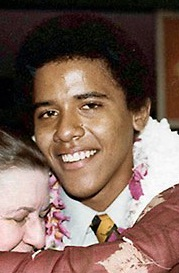
\includegraphics[width=0.25\textwidth]{obama4.png}
    \end{center}

    \begin{itemize}
      \pause
      \item We learn quickly from few, relatively unstructured examples
       ... but we don't understand {\it how} we accomplish this
      \item \alert<2>{Can we develop algorithms that enable machines
        to learn by example from large data sets?}
    \end{itemize}

\end{frame}

\begin{frame}
  \frametitle{Common applications}

  \begin{itemize}
    \item Effective/practical algorithms exist, and impact our daily lives
    \item Entire industries built around these techniques, e.g.:
      \begin{itemize}
        \item Spam detection (Email)
        \item Information retrieval (Search)
        \item Recommendation Systems (``You might also like ...'')
        \item Fraud detection (Identity theft)
        \item Face recognition (Camera auto-focus)
        \item Optical character recognition (Mail routing via ZIP codes)
      \end{itemize}
  \end{itemize}

\end{frame}


\begin{frame}
  \frametitle{Netflix prize}

    \begin{center}
      
\includegraphics[width=0.75\textwidth]{netflix.png}
    \end{center}

    \begin{itemize}
      \item \$1M for a 10\% improvement in predicted rating
      \item More than 1000 submissions over 2.5 years
      \item Top two teams within 0.01\% of each other (winners announced soon)
    \end{itemize}

\end{frame}


\begin{frame}
  \frametitle{Goals}

  \begin{itemize}
    \item Many fields ...
      \begin{itemize}
        \item Statistics
        \item Pattern recognition
        \item Data mining
        \item Machine learning
      \end{itemize}
    \item ... similar goals
      \begin{itemize}
        \item Extract and recognize patterns in data
        \item Interpret or explain observations
        \item Test validity of hypotheses
        \item Efficiently search the space of hypotheses
        \item Design efficient algorithms enabling machines to learn from data
      \end{itemize}
  \end{itemize}

\end{frame}

\begin{frame}
  \frametitle{Philosophy}

    \begin{itemize}
      \item We would like models that:
        \begin{itemize}
          \item Provide predictive and explanatory power
          \item Are complex enough to describe observed phenomena
          \item Are simple enough to generalize to future observations
        \end{itemize}

    \begin{center}
      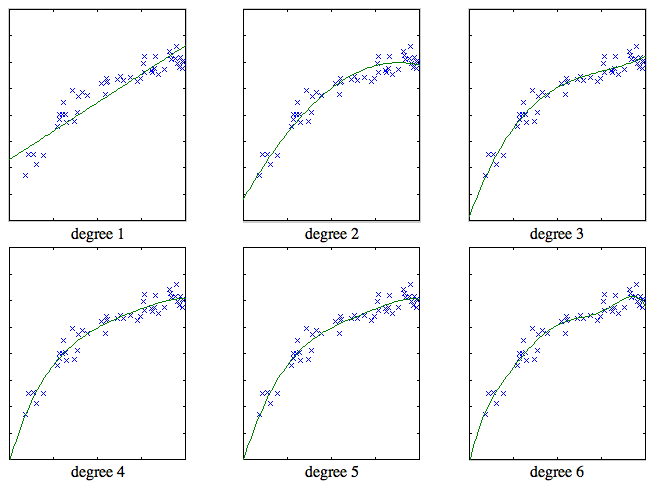
\includegraphics[width=0.5\textwidth]{regression.png}
    \end{center}


      \pause
      \item How can we quantify an ``optimal'' model
        \begin{itemize}
          \item What to optimize?
          \item How to optimize it?
        \end{itemize}

    \end{itemize}

\end{frame}


\begin{frame}
  \frametitle{Framework}

  \begin{columns}
    \begin{column}{0.6\textwidth}
      
  \begin{enumerate}
    \item<1-> Get data
    \item<2-> Visualize/perform sanity checks
    \item<2-> Clean/filter observations
    \item<2-> Choose features to represent data
    \item<3-> Specify model
    \item<3-> Specify loss function 
    \item<4-> Develop algorithm to minimize loss 
    \item<5-> Choose performance measure
    \item<5-> ``Train'' to minimize loss
    \item<5-> ``Test'' to evaluate generalization
  \end{enumerate}

    \end{column}
    \begin{column}{0.3\textwidth}

    \begin{center}
      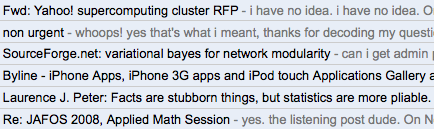
\includegraphics[width=0.9\textwidth]{email_ham.png}
      
\includegraphics[width=0.9\textwidth]{email_spam.png}
      \uncover<2-> {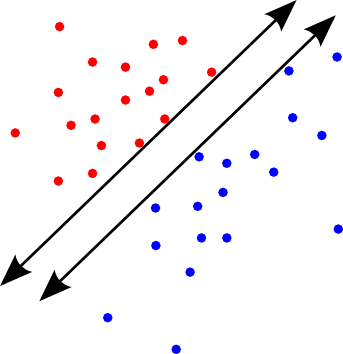
\includegraphics[width=0.5\textwidth]{svm.png}}
      \uncover<5-> {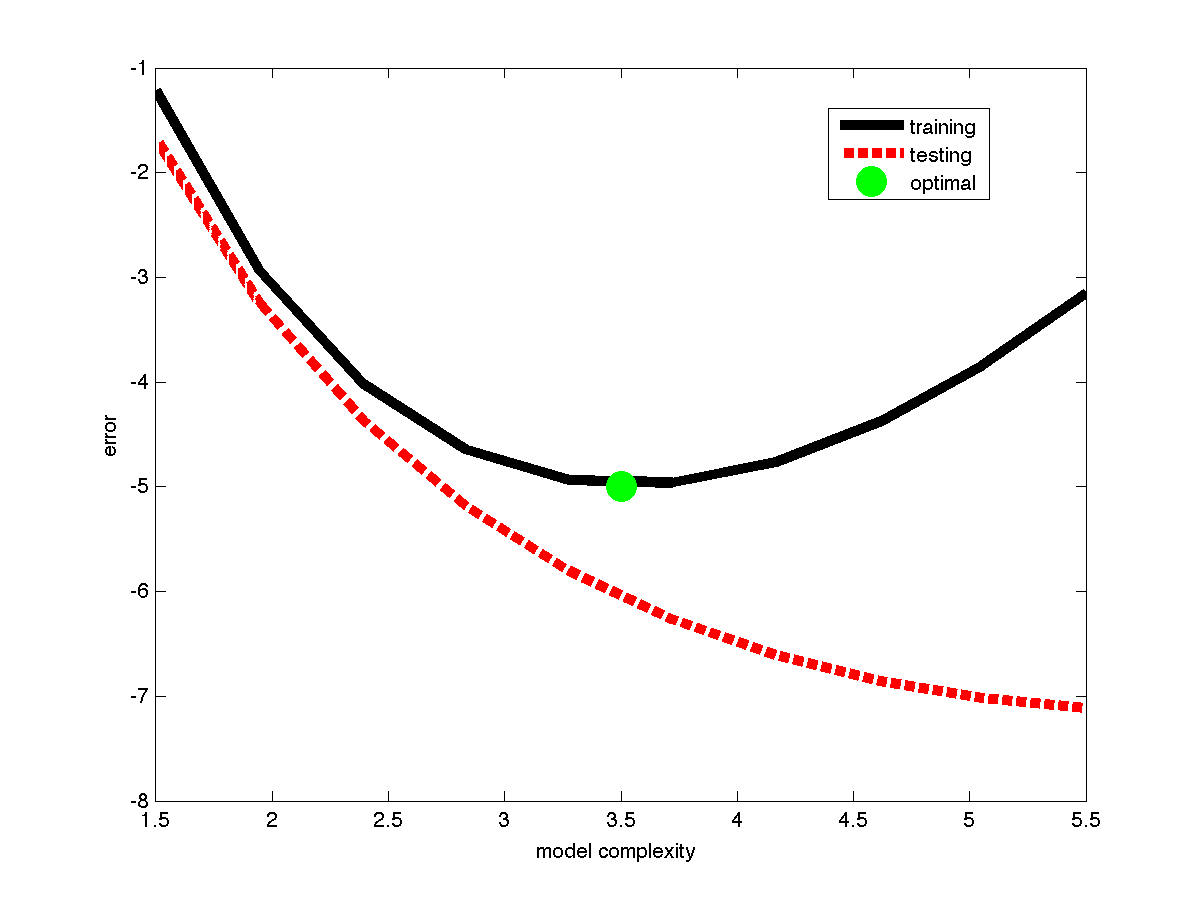
\includegraphics[width=0.9\textwidth]{complexity.png}}
    \end{center}

    \end{column}
  \end{columns}

% x=linspace(1.5,5.5,10);
% ytrain=x.^1.1-8*log(x);
% ytest=x.^1.5-10*log(x)+1;
% plot(x,ytrain,'r--','Linewidth',10)
% hold on
% plot(x,ytest,'k','Linewidth',5)
% plot(3.5,-5,'go','Linewidth',10)
% xlabel('model complexity')
% ylabel('error')
% legend('training','testing','optimal','location','best')

\end{frame}

\begin{frame}
  \frametitle{Topics}

  \begin{columns}[t]
    \begin{column}{0.5\textwidth}

      \begin{itemize}
      \item Supervised
        \begin{itemize}
          \item Linear regression
          \item Classification / regression trees
          \item Logistic regression
          \item Naive Bayes
          \item k-nearest neighbors
          \item Support vector machines
          \item Boosting
        \end{itemize}
      \end{itemize}

    \end{column}
    \begin{column}{0.5\textwidth}

      \begin{itemize}
      \item Unsupervised
        \begin{itemize}
          \item K-means
          \item Mixture models
          \item Principal components analysis
          \item Factor analysis
          \item Topic models
          \item Collaborative filtering
        \end{itemize}
      \end{itemize}

    \end{column}
  \end{columns}

  \pause
  \begin{itemize}
    \item Data representation: feature space, selection, normalization
    \item Model assessment: complexity control, cross-validation, ROC curve, Bayesian Occam's razor, information-theoretic measures
    \pause
    \item Probabilistic inference: graphical models, variational methods, sampling
    \item Large-scale learning (?)
  \end{itemize}

\end{frame}

\begin{frame}
  \frametitle{Topics}

  \begin{itemize}
    \item Simple approaches often do surprisingly well for large problems
  \end{itemize}

\end{frame}

\begin{frame}
  \frametitle{Got data?}

  \begin{itemize}
    \item Web service APIs expose vast amounts of data
  \end{itemize}

    \begin{center}
      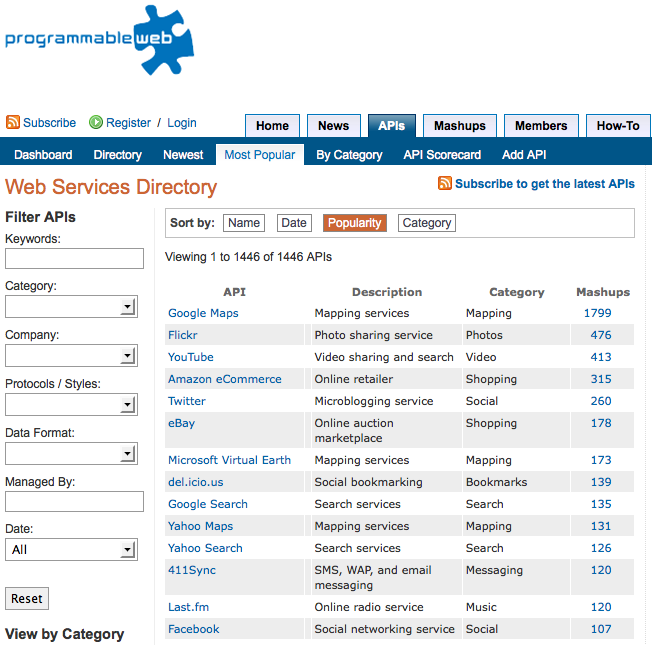
\includegraphics[width=0.625\textwidth]{programmableweb.png}
    \end{center}

\end{frame}

\begin{frame}
  \frametitle{Got data?}

  \begin{itemize}
    \item Many free, public data sets available online
  \end{itemize}

    \begin{center}
      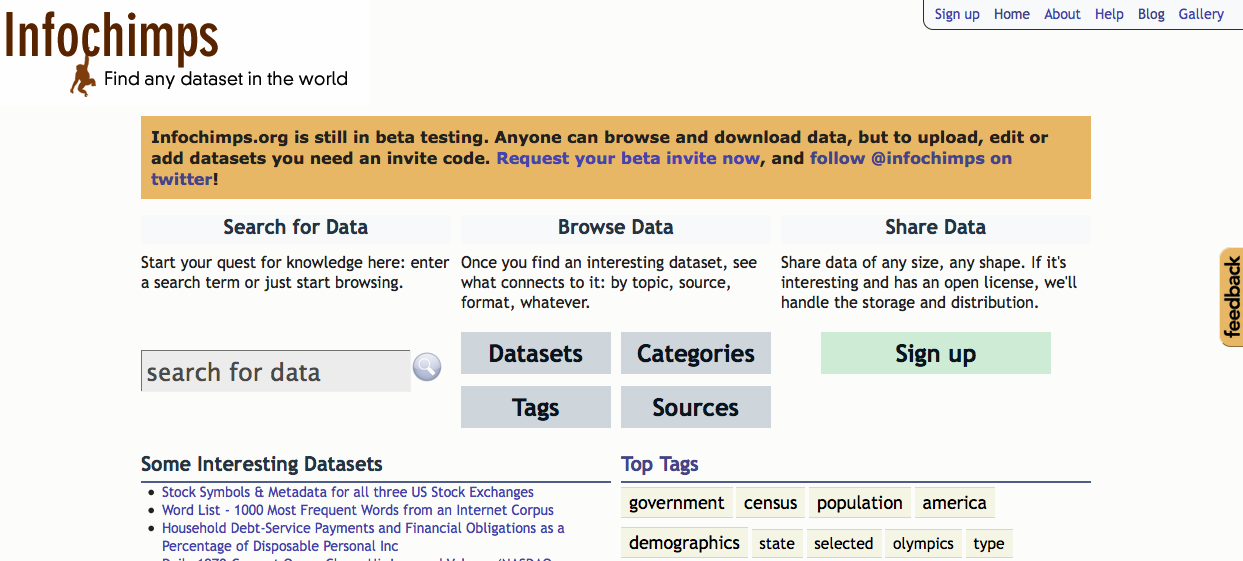
\includegraphics[width=0.9\textwidth]{infochimps.png}
    \end{center}

\end{frame}

\begin{frame}[fragile]
  \frametitle{Coding}

  \begin{itemize}
    \item Scripting: Python, Ruby, Perl, bash, ...
    \item Computing: R, SciPy/NumPy, MATLAB, ...
    \item Wrangling: sed, awk, grep, tr, wc, cut, sort, uniq, ....
  \end{itemize}

  \pause
  \begin{verbatim}
    $ tr , '\t' < data.csv > data.tsv
  \end{verbatim}

  \pause
  \begin{verbatim}
    $ bzcat data.tsv.bz2 | awk -F'\t' 'NF != 16 {print}'
  \end{verbatim}

  \pause
  \begin{verbatim}
    $ sed -e 's/<[^>]*>//g' < page.html > page.txt
  \end{verbatim}


\end{frame}

% section motivation_for_bootcamp (end)

\end{document}
